\documentclass[a4paper]{article}
\usepackage[14pt]{extsizes}
\usepackage[utf8]{inputenc}
\usepackage[T2A]{fontenc}
\usepackage[russian]{babel}
\usepackage{setspace,amsmath}
\usepackage{amssymb, amsthm}
\usepackage{graphicx}
\usepackage{mathtext}
\usepackage{mathenv}
\usepackage{tocloft}
\usepackage{enumitem}
\usepackage[indentfirst]{titlesec}
\usepackage[left=30mm, top=20mm, right=20mm, bottom=20mm, nohead, footskip=10mm]{geometry}

\onehalfspacing

\makeatletter
\renewcommand{\cftsecleader}{\cftdotfill{\cftdotsep}}

\newtheorem*{mproblem}{Условие}
\newtheorem*{mclaim}{Утверждение}
\newtheorem*{mremark}{Замечание}
\newtheorem*{mdefinition}{Определение}
\newtheorem*{mlemma}{Лемма}
\newtheorem*{mtheorem}{Теорема}
\newtheorem*{msolution}{Доказательство}

\begin{document}
\begin{titlepage}
	\begin{center}
		\hfill \break
		\large{Министерство образования и науки Российской Федерации}\\
		\hfill \break
		\normalsize{Государственное образовательное учреждение}\\ 
		\normalsize{высшего профессионального образования}\\
		\normalsize{«Московский физико-технический институт (государственный университет)»}\\
		\normalsize{Факультет инноваций и высоких технологий}\\
		\normalsize{Кафедра анализа данных}\\
		\hfill \break
		\hfill \break
		\hfill \break
		\Large{\textbf{Магистерская диссертация}}\\
		\hfill \break
		\large{Тема: \textbf{Название моей работы (TODO)}}\\
	\end{center}

	\begin{flushright}
		\hfill \break
		Направление:  010400\\
		Прикладные математика и информатика\\
		\hfill \break
		\hfill \break
		\hfill \break
	\end{flushright}
	
	\begin{flushright}
		\normalsize{
			\begin{tabular}{rcr}
				Выполнил:\ \\ студент 093 группы & \underline{\hspace{3cm}} & Попов М.В. \\\\
				Научный руководитель:\ \\ д.физ.-мат.н., проф.(todo) & \underline{\hspace{3cm}}& Ромащенко А.Е. \\\\
			\end{tabular}
		}
	\end{flushright}

	\begin{center}
		\hfill \break
	\end{center}

	\begin{center} г. Москва 2016 \end{center}
	\thispagestyle{empty}
\end{titlepage}
 
\newpage

\tableofcontents

\newpage
 
\newpage


\setcounter{section}{0}
\section*{Введение}
\addcontentsline{toc}{section}{Введение}
(ToDo) Актуальность, новизна, краткая выжимка.

\addtocounter{section}{1}
\section*{Коммуникационная сложность}
\addcontentsline{toc}{section}{Коммуникационная сложность}
\setcounter{subsection}{0}

\subsection{Постановка задачи}
Мы будем рассматривать задачи следующего вида: пусть имеется два человека, которые хотят совместно
вычислить значение некоторой функции от двух переменных $f(x, y)$. По традиции мы будем называть
первого участника игры Алисой, а второго Бобом. Сложность у этой задачи в том, что Алиса знает только
значение аргумента $x$, а Боб значение аргумента $y$. Алиса и Боб могут обмениваться сообщениями 
по каналу связи. Требуется вычислить значение $f(x, y)$, переслав по каналу связи минимальное
количество информации.

Мы предполагаем, что Алиса и Боб заранее (до того, как им станут известны значения $x$ и $y$)
договариваются о коммуникационном протоколе --- о наборе соглашений, какие именно данные и
в каком порядке они будут пересылать друг другу при тех или иных значениях $x$ и $y$.

Опишем теперь всю задачу более формально. Пусть имеются конечные множества $X, Y, Z$ и задана
некоторая функция $f:X\times Y\rightarrow Z$.

\begin{mdefinition}
    Коммуникационным протоколом для вычисления некоторой функции $f:X\times Y\rightarrow Z$ называется
    ориентированное двоичное дерево со следующей разметкой на вершинах и ребрах:
    \begin{itemize}[noitemsep]
        \item каждая нелистовая вершина помечена буквой $A$ или $B$;
        \begin{itemize}[noitemsep]
			\item у вершин с пометкой $A$ определена функция $g_i:X\rightarrow \{0,1\}$;
			\item у вершин с пометкой $B$ определена функция $f_j:Y\rightarrow \{0,1\}$;
        \end{itemize}
        \item каждой листовой вершине сопоставлен элемент множеста $Z$;
        \item каждое ребро помечено $0$ или $1$.

    \end{itemize}
\end{mdefinition}

Пусть Алиса и Боб договорились, что будут действовать по некоторому протоколу $\mathcal{P}$. Затем
Алиса получила $x\in X$, а Боб получил $y\in Y$. Поместим фишку в корневую вершину нашего протокола
$\mathcal{P}$ и будем перемещать ее вниз по дереву, последовательно удаляясь от корня,
пока она не попадём в один из листьев. Перемещение фишки выполняется следующим образом. Если текущая 
вершина помечена буквой $A$ это значит, что сейчас очередь Алисы. Она применяет функцию $g_i$ текущей 
вершины к своему значению $x$. Алиса отправляет по каналу связи бит равный $g_i(x)$ и перемещает
фишку по ребру, помеченному как $g_i(x)$. Боб получает отправленный бит и понимает куда была сдвинута фишка.
Для вершин помеченных буквой $B$ поступают аналогично. Когда фишка попадает в лист дерева,
записанное там значение $z\in Z$ объявляется результатом выполнения протокола.

Мы говорим, что протокол $\mathcal{P}$ вычисляет функцию $f:X\times Y \rightarrow Z$, если для любого
$x\in X$ и любого $y\in Y$ при движении из корня по пути, соответствующему заданным $x$ и $y$,
мы попадаем в лист, помеченный $z=f(x,y)$.

\begin{mdefinition}
	Сложностью коммуникационного протокола называется его глубина. Коммуникационной сложностью функции 
	$f$ называется минимальная сложность протокола, вычисляющего $f$. Мы будем обозначать её $CC(f)$.
\end{mdefinition}


\subsection{Одноцветные комбинаторные прямоугольники}
\begin{mdefinition}
	Множество $S \subset X\times Y$ называется комбинаторным прямоугольником (или просто прямоугольным
	множеством), если существуют такие $A \subset X$ и $B \subset Y$, что $S = A\times B$.
\end{mdefinition}

Пусть $\mathcal{P}$ некоторый коммуникационный протокол для вычисления функции $f:X\times Y \rightarrow Z$ 
и $l$ один из листьев протокола. Определим $S_l$, как множество пар $(x, y) \in X\times Y$ таких, что 
на входе $(x,y)$ Алиса и Боб, следуя протоколу $\mathcal{P}$, приходят в лист $l$.

\begin{mclaim}
    Для всякого коммуникационного протокола $\mathcal{P}$ и для всякого листа $l$ множество $S_l$
    является комбинаторным прямоугольником. 
\end{mclaim}

Доказательсво этого утверждения можно прочитать например в \cite{KushilevitzNisan}. В итоге мы получаем,
что коммуникационный протокол для вычисления функции $f$ задаёт разбиение $X\times Y$ - 
таблицы значений $f$ на прямоугольные множества, соответствующие листьям. Поскольку каждому
листу протокола приписано одно значение функции $f$, эти прямоугольные множества являются одноцветными,
то есть во всех точках такого прямоугольного множества функция $f$ принимает одно и то же значение.
Например, для $X = Y = \{1, 2, 3, 4\}$, $Z = \{0, 1\}$ и протокола $\mathcal{P}$ (рис 1.) получаем 
разбиение на $5$ одноцветных прямоугольных множества. 

\begin{figure}
	\centering
	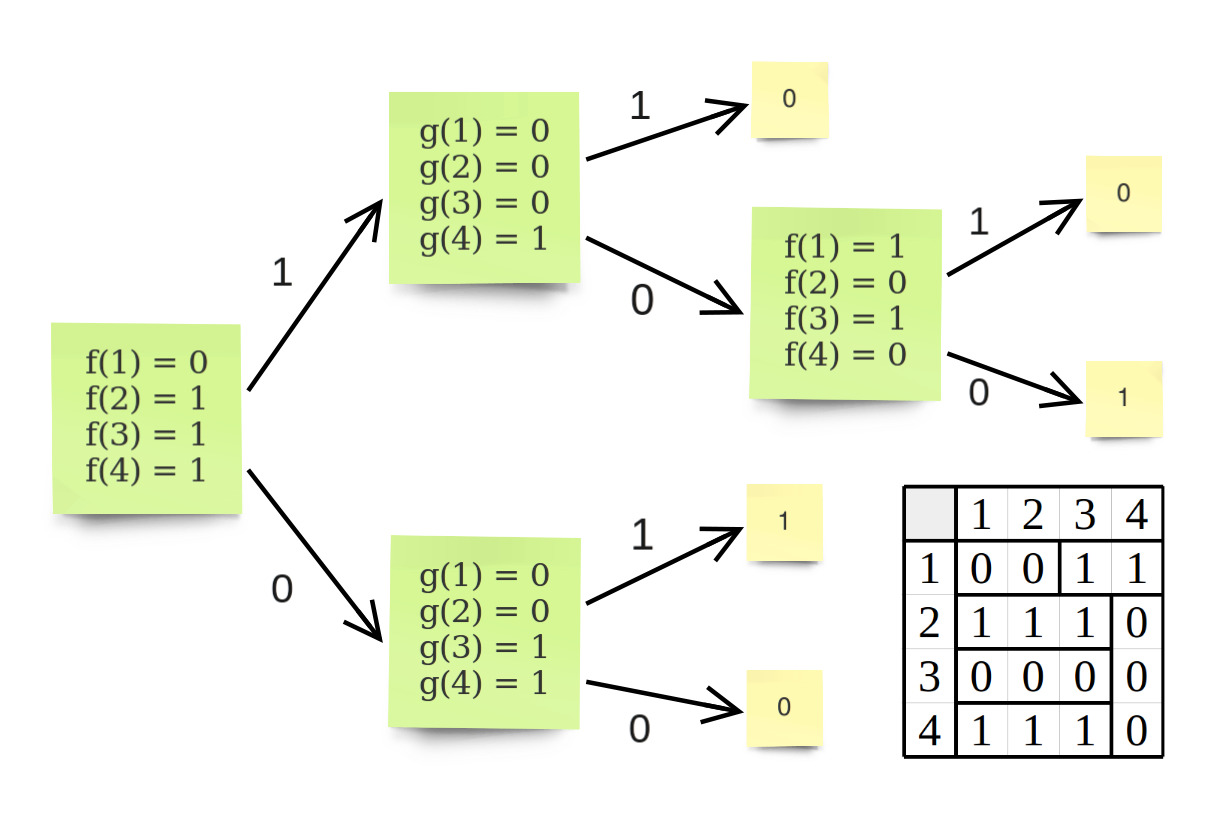
\includegraphics[width=0.8\textwidth]{images/protocol.png}
	\caption{Пример протокола и разбиения таблицы значений.}
\end{figure}

Подведем промежуточные итоги: всякий протокол с $l$ листьями (вычисляющий функцию $f$) задаёт разбиение
таблицы значений $f$ на $l$ одноцветных прямоугольных множества. Значит, чтобы доказать, что коммуникационная 
сложность $CC(f)$ не меньше $n$, достаточно показать, что таблицу значений невозможно разбить на менее,
чем $2^n$ одноцветных прямоугольных множества.

\subsection{Графовая интерпретация}

Давайте теперь посмотрим на другое представление множества значений функции $f$. Рассмотрим полный 
двудольный граф $G = (X, Y, E)$, ребра которого раскрашены в $|Z|$ цветов. Вершины левой доли 
соответствуют элементам множества $X$, вершины правой доли - элементам множества $Y$. Ребро 
$(x, y) \in X\times Y$ имеет цвет $z \in Z$, если $f(x, y) = z$.

Из определения комбинаторного прямоугольника видно, что в графовой интерпертации он является ничем
иным, как полным двудольным подграфом. А разбиение таблицы значений $f$ на одноцветные прямоугольные
множества это разбиение нашего  полного двудольного графа $G$ на одноцветные непересекающиеся биклики 
(полные двудольные подграфы). Для нашего примера графовую интерпретацию можно посмотреть на рис.2.

\begin{figure}
	\centering
	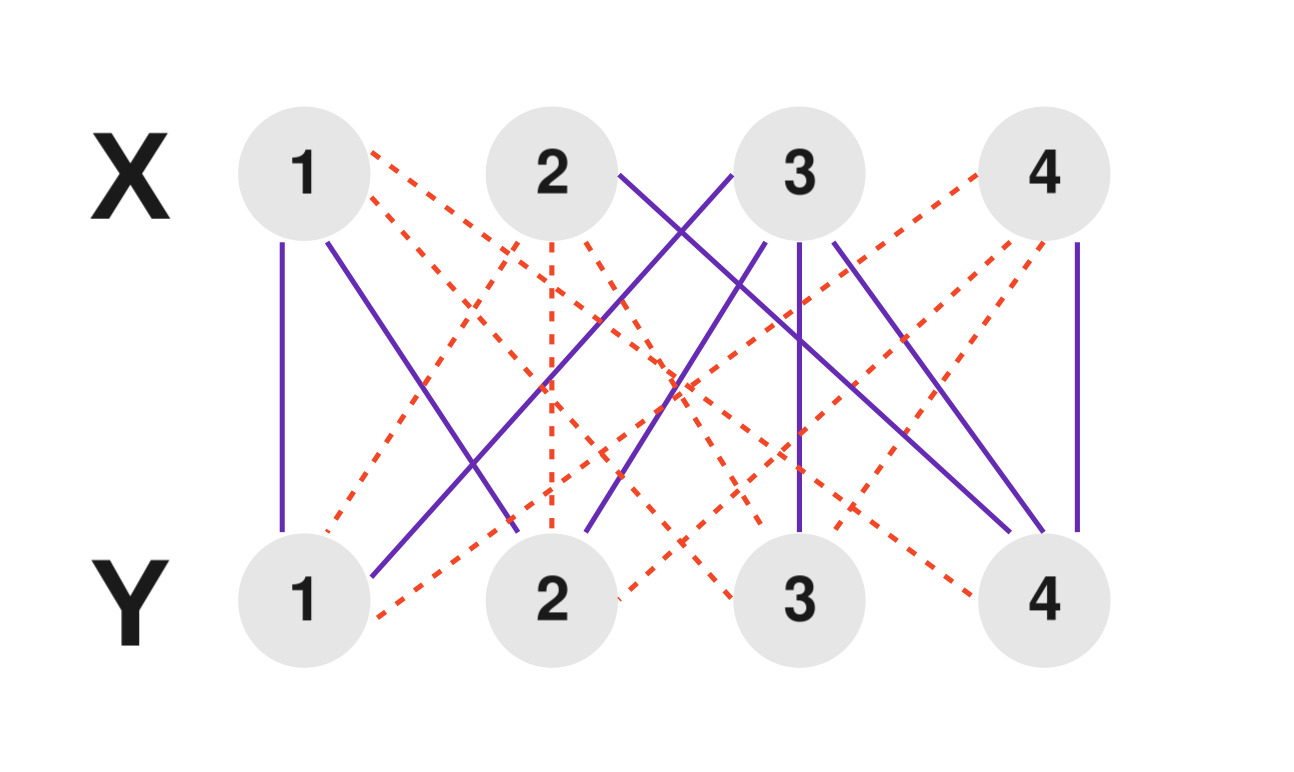
\includegraphics[width=0.6\textwidth]{images/biclique.png}
	\caption{Графовая интерпретация: синие -- 0, красные -- 1.}
\end{figure}

\begin{mdefinition}
	Бикликовым числом $bcc(G)$ двудольного графа $G$ будем называть наименьшее число биклик, которыми 
	можно покрыть все ребра графа $G$ (Биклики могут пересекаться).
\end{mdefinition}

Для каждого $z \in Z$ определим двудольный граф $G_z = (X, Y, E_z)$, как граф, получающийся из $G$ 
выкидыванием всех ребер цвета отличного от $z$, иначе говоря $E_z = \{(x,y)\in X\times Y\ |\ f(x, y) = z \}$.

Величины $bbc(G_z)$ дают некоторую нижнюю оценку на величину минимального покрытия непересекающимися 
бикликами, поэтому: $$2^{CC(f)}\geq \sum\limits_{z\in Z}bcc(G_z)$$

\begin{mremark}
    На самом деле величины $bbc(G_z)$ тесно связаны с недетерминированной коммуникационной сложностью 
    $NCC(f)$. Для произовльного множества $Z$ верно: 
    $$NCC(f) \leq \lceil log_2(\sum\limits_{z\in Z}bcc(G_z))\rceil + 1$$ а для 
    $Z = \{0, 1\}$: $$NCC(f) = \lceil log_2(bcc(G_1))\rceil$$ 
    Подробнее про это можно прочитать, например в \cite{Razborov}.
\end{mremark}

В итоге мы получили мощный иструмент для доказательства нижних оценок коммуникационной сложности. 
К сожалению задача нахождения величины $bcc(G)$ является PSPACE-полной \cite{HermannMarkus}, а точное 
значение известно только для очень скудного класса графов (например для "Crown graphs"), поэтому 
напрямую мы не можем использовать эту оценку. В следующей главе я рассмотрю несколько методов, 
позволяющих для произвольного двудольного графа оценивать снизу величину $bcc(G)$.


\addtocounter{section}{1}
\section*{Оценивание $bcc(G)$}
\addcontentsline{toc}{section}{Оценивание $bcc(G)$}

В этой главе я опишу три различных метода оценивания бикликового покрытия:
\begin{itemize}[noitemsep]
	\item метод трудного множества ("Fooling Set");
	\item метод Куликова-Юкны;
	\item метод энтропийных неравенств.
\end{itemize}

Первые два метода работают для произвольных графов (необязательно двудольных), а третий применим к 
большому классу двудольных графов.

\setcounter{subsection}{0}

\subsection{Метод трудного множества}

Данный метод тесно связан с одноцветными прямоугольными множествами. Классическое определение 
трудного множества выглядит следующим образом:

\begin{mdefinition}
	Для функции $f: X\times Y \rightarrow Z$ и элемента $z\in Z$ будем называть множество 
	$S_z\subset X\times Y$ трудным (в англоязычной литературе fooling set), если верно:
	\begin{itemize}[noitemsep]
		\item для всякой пары $(x, y)\in S_z$ имеем $f(x, y) = z$;
		\item для любых двух несовпадающих пар $(x, y)\in S_z$ и $(x', y')\in S_Z$ имеем 
		$f(x, y') \neq z$ или $f(x', y) \neq z$.
	\end{itemize}
\end{mdefinition}

Нас будет интересовать немного более общее определение трудного множества (графовая интерпретация):
\begin{mdefinition}
	Пусть $G = (V, E)$ произвольный неориентированный граф. Будем называть подмножество ребер 
	$S \subseteq E$ трудным, если для любых двух различных ребер $(x, y)\in S$ и $(x', y')\in S$ 
	имеем $(x, y') \notin E$ или $(x', y) \notin E$.
\end{mdefinition}

\begin{mremark}
	Классическое определение получается из графового, применением к двудольному графу $G_z = (X, Y, E_z)$, 
	который строится по функции $f: X\times Y \rightarrow Z$.
\end{mremark}

	
\begin{mtheorem}
    Для произвольного неориентированного графа $G = (V, E)$, если подмножество ребер $S \subseteq E$ 
    является трудным, то $bcc(G) \geq |S|$.
\end{mtheorem}

\begin{msolution}
    Достаточно доказать, что два ребра, лежащие одновременно в одном трудном множестве, не могут 
    попасть в одну биклику. Пусть не так, значит существуют два ребра $(x, y)\in B\cap S$ и 
    $(x', y')\in B\cap S$, где $B$ - биклика, а $S$ - трудное подмножество ребер. Но тогда ребра 
    $(x, y')$ и $(x', y)$ также принадлежат биклике $B$, а значит лежат и в нашем множестве ребер 
    $E$. Противоречие. $\blacksquare$
\end{msolution}

\begin{mremark}
    На практике нахождение максимального по мощности трудного множества применяют редко, потому что 
    эта задача является $PSPACE$-полной \cite{HermannMarkus}. Часто рассматривают "нечестный"\ метод, 
    а именно доказывают, что определенного размера трудное множество обязательно найдется.
\end{mremark}

\begin{mtheorem}
    Для произвольного неориентированного графа $G = (V, E)$ обозначим за $v(G)$ - размер максимального 
    паросочетания, а за $cl(G)$ такое максимальное число $r$, что в нашем графе содержится биклика 
    $K_{r,r}$. Тогда среди ребер этого паросочетания можно найти трудное множество размера 
    $\Big\lceil\frac{v(G)}{cl(G)}\Big\rceil$. 
\end{mtheorem}

На самом деле намного проще доказать, что $bcc(G) \geq \Big\lceil\frac{v(G)}{cl(G)}\Big\rceil$ 
без участия трудного множества. Этот факт сразу следует из того, что любая биклика $K_{r, s}$ 
содержит как максимум $min\{r, s\}$ ребер максимального паросочетания. Сама теорема будет доказана 
в одной из последующих глав.

\subsection{Метод Куликова-Юкны}
Следующий метод был впервые описан в статье \cite{KulikovJukna} и работает он для произвольного 
неориентированного графа.

\begin{mtheorem}
    Для произвольного неориентированного графа $G = (V, E)$ верно: $$bcc(G)\geq \bigg\lceil\frac{v(G)^2}{|E|}\bigg\rceil$$
\end{mtheorem}

\begin{msolution}
	Пусть $M\subseteq E$ - это максимальное паросочетание, тогда рассмотрим бикликовое покрытие, 
	на котором достигается минимум $E = B_1\cup B_2\cup \ldots \cup B_{bcc(G)}$. Определим 
	отображение $g:M\rightarrow \{1,\ \ldots,\ bcc(G)\}$, как $g(e) = min\{i\ |\ e\in B_i\}$ и пусть 
	$M_i = \{e\in M\ |\ g(e) = i\}$. Иначе говоря $M_i$ содержит только те ребра максимального 
	паросочетания $M$, которые покрываются бикликой $B_i$ впервый раз.
	
	Пусть $F_i \subseteq B_i$ биклика, индуцированная вершинами ребер из $M_i$. Пусть 
	$F = F_1\sqcup F_2\sqcup \ldots \sqcup F_{bcc(G)}$ (биклики $F_i$ не пересекаются по построению).
	
	Очевидно, что $F_i$ - биклика размера $r_i\times r_i$, где $r_i = |M_i|$. Получаем следующие 
	соотношения: $$r_1 + r_2 + \ldots + r_{bcc(G)} = |M| = v(G)$$ и 
	$$r_1^2 + r_2^2 + \ldots + r_{bcc(G)}^2 = |F|$$ Из неравенства Коши-Буняковского получаем 
	$$v(G)^2 = (r_1 + r_2 + \ldots + r_{bcc(G)})^2 \leq bcc(G)\cdot (r_1^2 + r_2^2 + \ldots + r_{bcc(G)}^2) = bcc(G)\cdot |F|$$
	А так как $F \subseteq E$, то $v(G)^2\leq bcc(G)\cdot |F| \leq bcc(G)\cdot |E|$. 
	$\blacksquare$
\end{msolution}

На некоторых графах данная оценка превосходит $\Big\lceil\frac{v(G)}{cl(G)}\Big\rceil$, 
а на некоторых уступает:
\begin{itemize}
    \item пусть двудольный граф $G = (L, R, E)$ состоит из совершенного паросочетания размера 
    $n = |L| = |R|$ и еще некоторого константного числа непересекающихся биклик $K_{r,r}$. 
    К тому же, пусть $r = \Theta(\sqrt{n})$, тогда $$\frac{v(G)^2}{|E|} = \frac{n^2}{cr^2 + n} = 
    \Theta(n) \gtrsim \Theta(\sqrt{n}) = \frac{n}{r} = \frac{v(G)}{cl(G)}$$ 
    \item рассмотрим двудольный граф Леви, построенный при помощи конечной проективной плоскости порядка 
    $p\in \mathbb{P}$. В каждой доле этого графа содержится $n = p^2 + p + 1$ вершин, причем степень 
    каждой $p+1$. Этот граф не содержит $K_{2,2}$ (любые две прямые пересекаются максимум в одной точке). 
    А так как в регулярных двудольных графах обязательно найдется совершенное паросочетание, то 
    $$\frac{v(G)^2}{|E|} = \frac{(p^2 + p + 1)^2}{(p^2+p+1)(p+1)} = \Theta(\sqrt{n}) \lesssim 
    \Theta(n) = \frac{p^2 + p + 1}{1} = \frac{v(G)}{cl(G)}$$
\end{itemize}




\subsection{Метод энтропийных неравенств}




\addcontentsline{toc}{section}{Список литературы}
\bibliographystyle{utf8gost705u}
\bibliography{biblio}
\end{document}
